In this section, the layer is described in some detail in terms of its specific subsystems. Describe each of the layers and its subsystems in a separate chapter/major subsection of this document. The content of each subsystem description should be similar. Include in this section any special considerations and/or trade-offs considered for the approach you have chosen.



\begin{figure}[h!]
	\centering
 	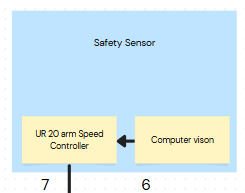
\includegraphics[width=0.60\textwidth]{images/safety_sens}
 \caption{Example subsystem description diagram}
\end{figure}

\subsection{UR 20 arm speed controller}
The controller will determine whether there is a person within the working vicinity of the UR20 robot and signal the PLC to adjust for the case
\subsubsection{Assumptions}
The UR20 should have collision detection and should stop at impact

\subsubsection{Responsibilities}
To signal the PLC the presence of a person near the robot using a computer vision algorithm

\subsubsection{Subsystem Interfaces}


\begin {table}[H]
\caption {Speed Controller Subsystem Interface} 
\begin{center}
    \begin{tabular}{ | p{1cm} | p{6cm} | p{3cm} | p{3cm} |}
    \hline
    ID & Description & Inputs & Outputs \\ \hline
    \#06 & send signal & \pbox{3cm}{presence detection} & \pbox{3cm}{presence signal}  \\ \hline
    \end{tabular}
\end{center}
\end{table}

\subsection{Computer vision algorithm}
A computer vision algorithm to scan for the presence of a person being near the UR20 robot
\subsubsection{Assumptions}
assume that the camera has a good point of view as to beable to see all around the robot 

\subsubsection{Responsibilities}
Inform controller of detected pressence near the UR20 

\subsubsection{Subsystem Interfaces}


\begin {table}[H]
\caption {Computer Vision Subsystem Interface} 
\begin{center}
    \begin{tabular}{ | p{1cm} | p{6cm} | p{3cm} | p{3cm} |}
    \hline
    ID & Description & Inputs & Outputs \\ \hline
    \#07 & presence detection & \pbox{3cm}{camera reading} & \pbox{3cm}{presence detection}  \\ \hline
    \end{tabular}
\end{center}
\end{table}

